\documentclass[12pt, table]{beamer}
\usetheme{Darmstadt}
\usepackage{graphicx}
%\usepackage[german]{babel}
\usepackage{ngerman}
\usepackage[T1]{fontenc}
\usepackage[utf8]{inputenc}
\usepackage{tikz}
\usepackage{csquotes}
\usepackage{hyperref}
\usepackage[shadow,colorinlistoftodos]{todonotes}
\usepackage{enotez}


\usepackage{adjustbox}
\usepackage{booktabs}

% <https://tex.stackexchange.com/questions/32683/rotated-column-titles-in-tabular>
\newcolumntype{R}[2]{%
>{\adjustbox{angle=#1,lap=\width-(#2)}\bgroup}%
 l%
<{\egroup}%
}
\newcommand*\rot{\multicolumn{1}{R{70}{1em}}}

\setbeamertemplate{footline}[frame number]

\newcommand{\cc}[1]{\includegraphics[height=4mm]{../img/#1.png}\hspace{1mm}}
\usepackage{ifthen}
\newcommand{\license}[2][]{\\#2\ifthenelse{\equal{#1}{}}{}{\\\scriptsize\url{#1}}}
\usepackage{textcomp}
\usepackage{hyperref}

\pgfdeclareimage[height=.6cm]{c3d2logo}{../img/c3d2.pdf}

\pgfdeclarelayer{foreground}
\pgfsetlayers{main,foreground}
\logo{\pgfputat{\pgfxy(-1,0)}{\pgfbox[center,base]{\pgfuseimage{c3d2logo}}}}

\setbeamercovered{transparent}

\title{Digitale Selbstverteidigung}
\author{\small nac\\\large Chaos Computer Club Dresden}
\date{30.05.2018}

\begin{document}

\section{Intro}
\subsection{}

\begin{frame}
	\frametitle{Intro}
	\begin{center}
		
\includegraphics[height=0.5\textheight]{../img/cms-text.png}
	\end{center}
\end{frame}

\begin{frame}
\frametitle{Wer sind wir?}
	\begin{center}
		\only<1>{
			\begin{center}
				
\includegraphics[height=0.1\textheight]{../img/c3d2_logo.png}
			\end{center}
			}
		\only<2>{
			\begin{center}
				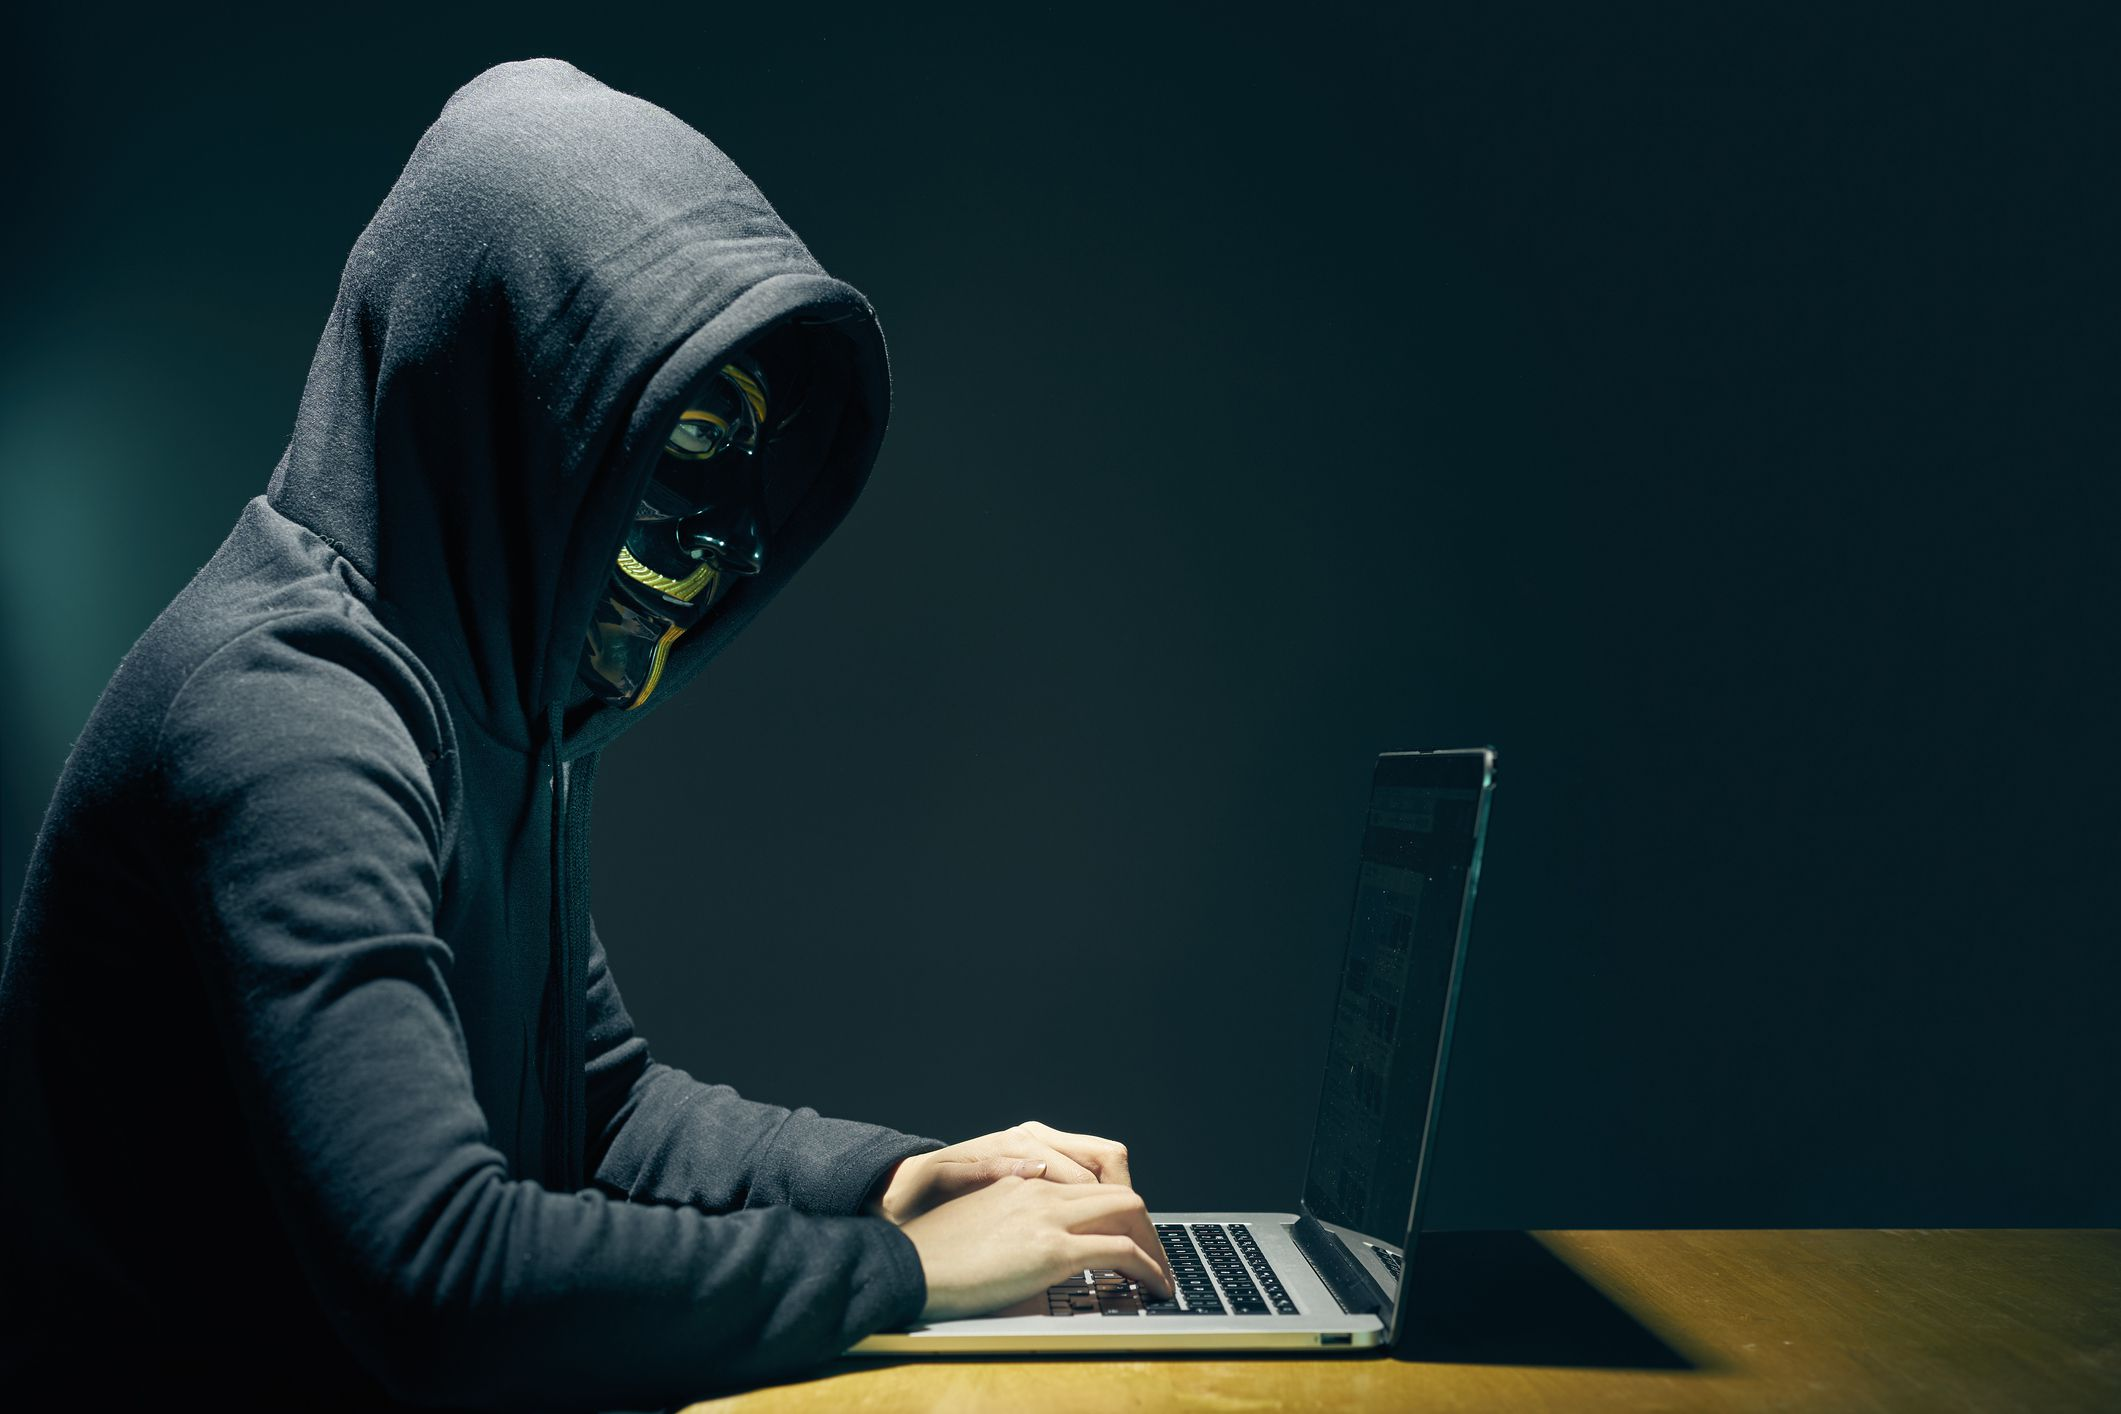
\includegraphics[height=0.7\textheight]{../img/hacker.jpg}
			\end{center}
			}
		\only<3>{
			\begin{center}
				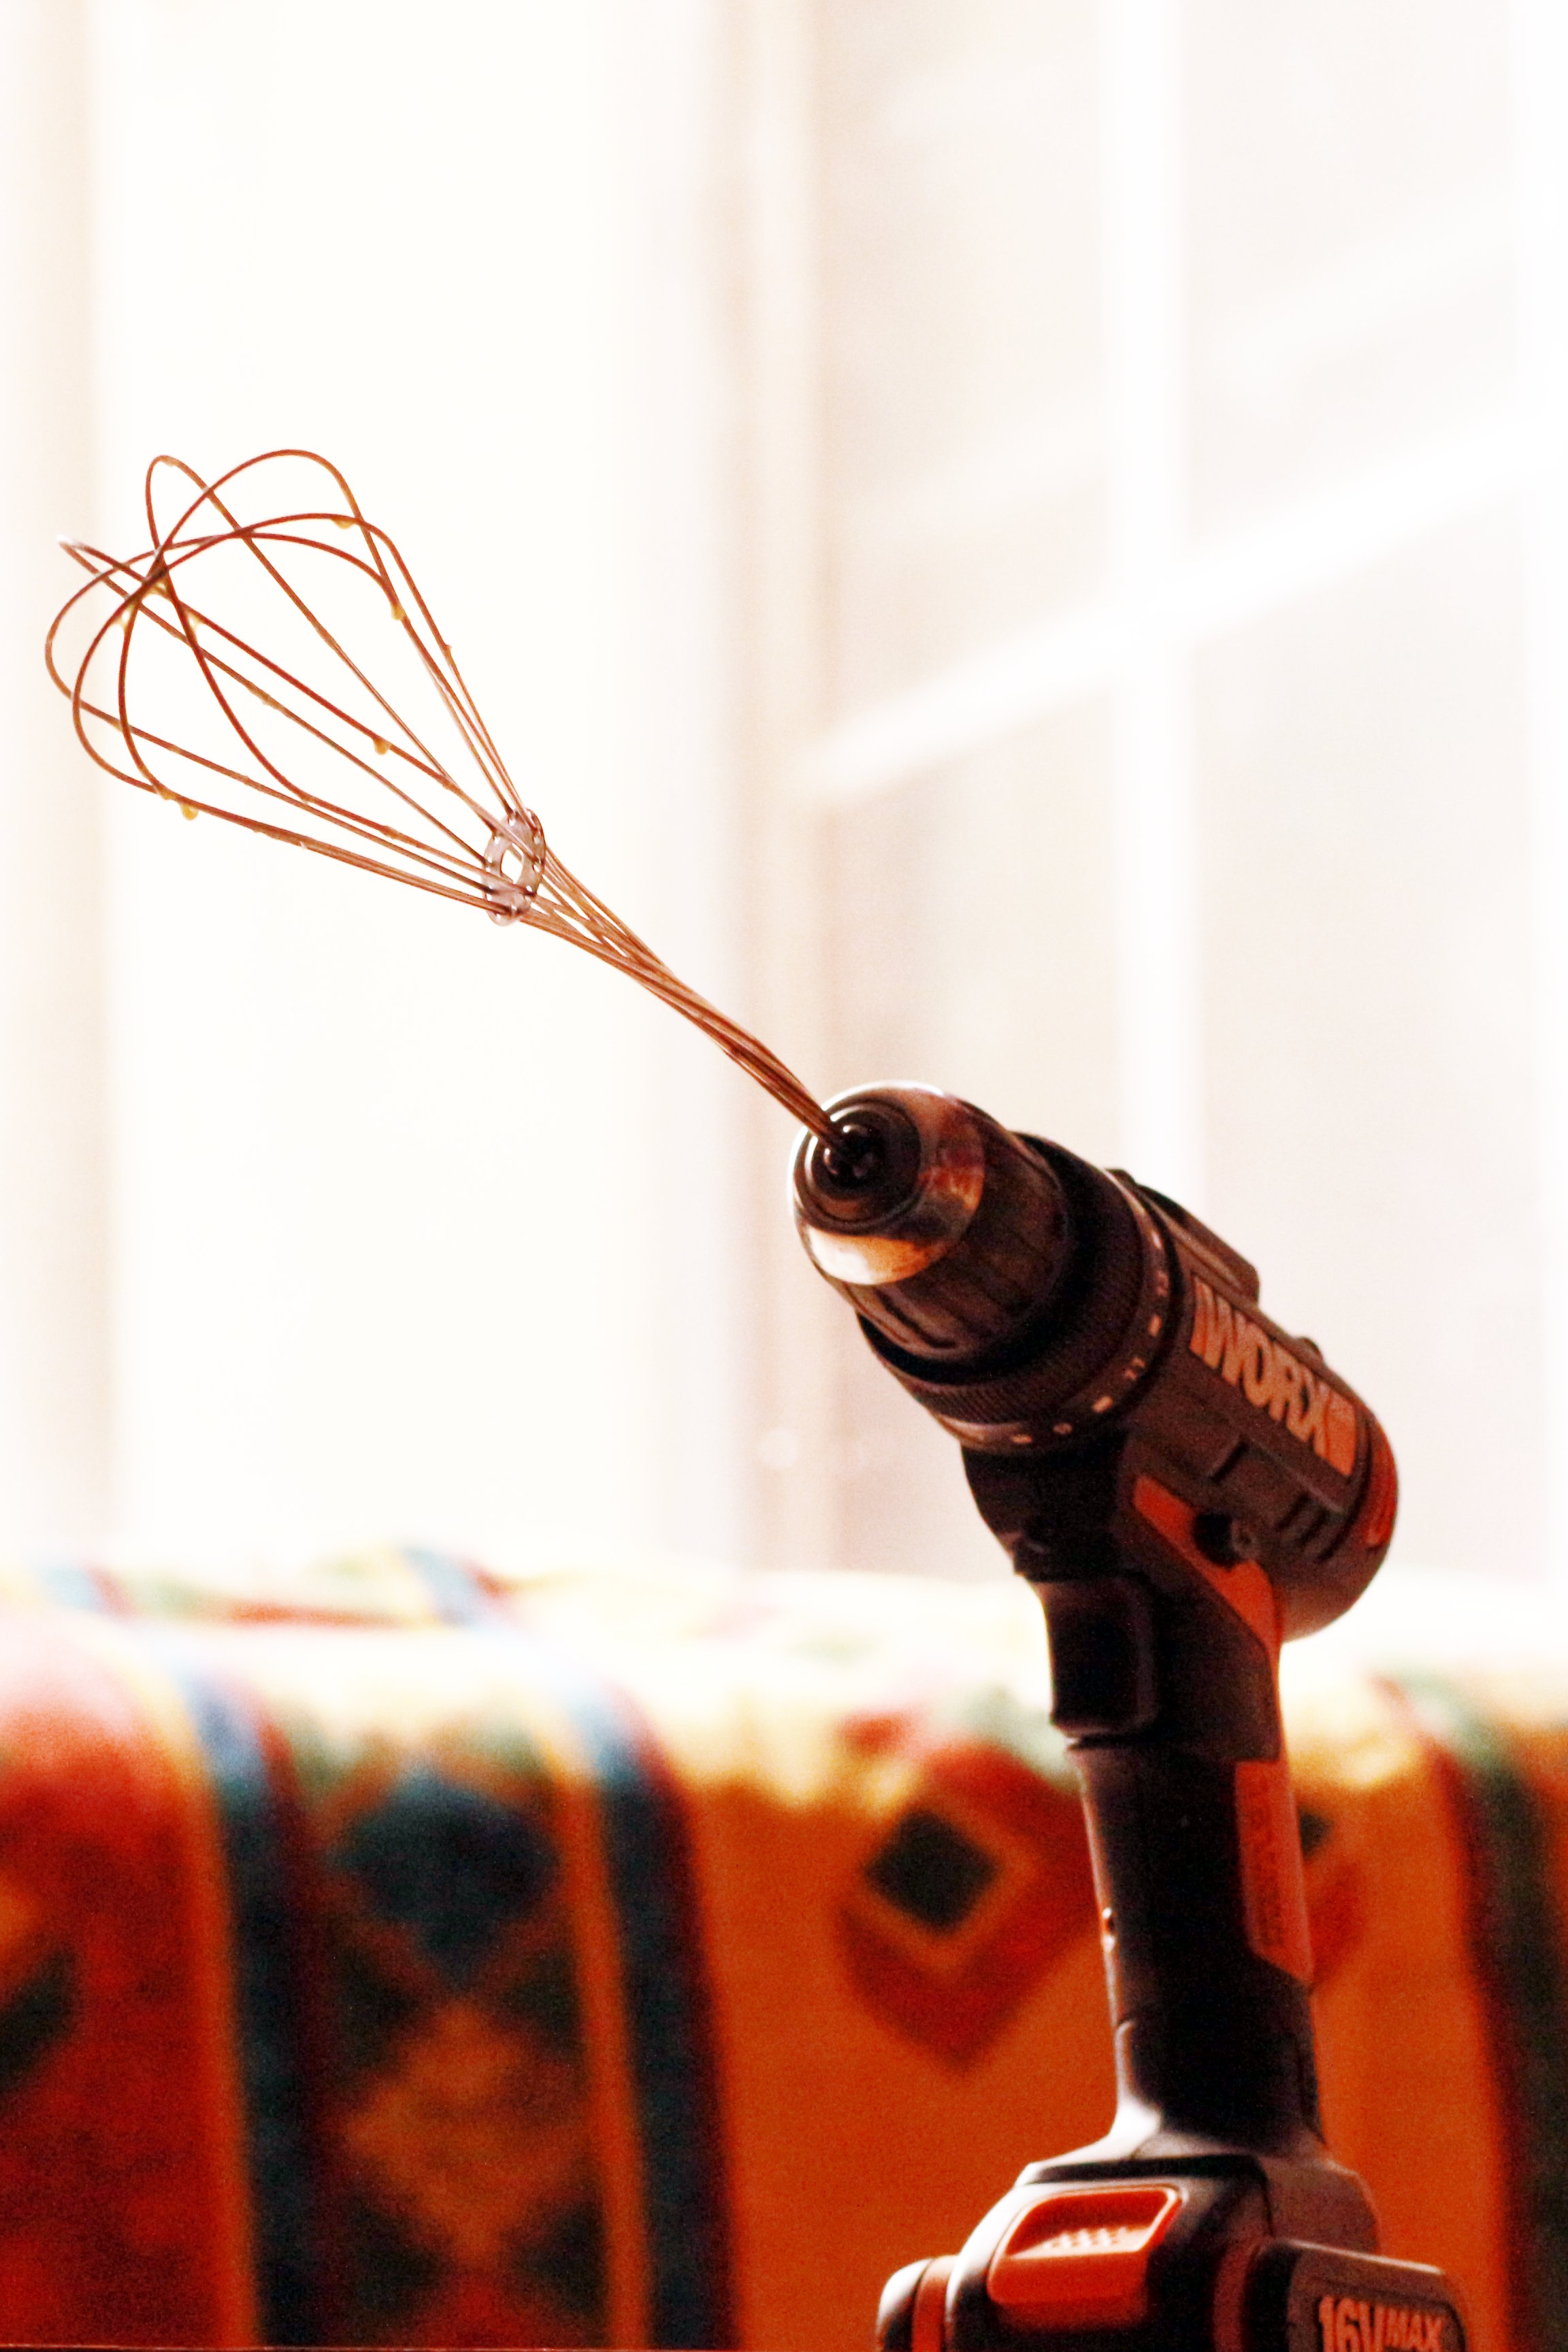
\includegraphics[height=0.7\textheight]{../img/schneeschrauber.jpg}
			\end{center}
			}
		\only<4>{
			\begin{center}
				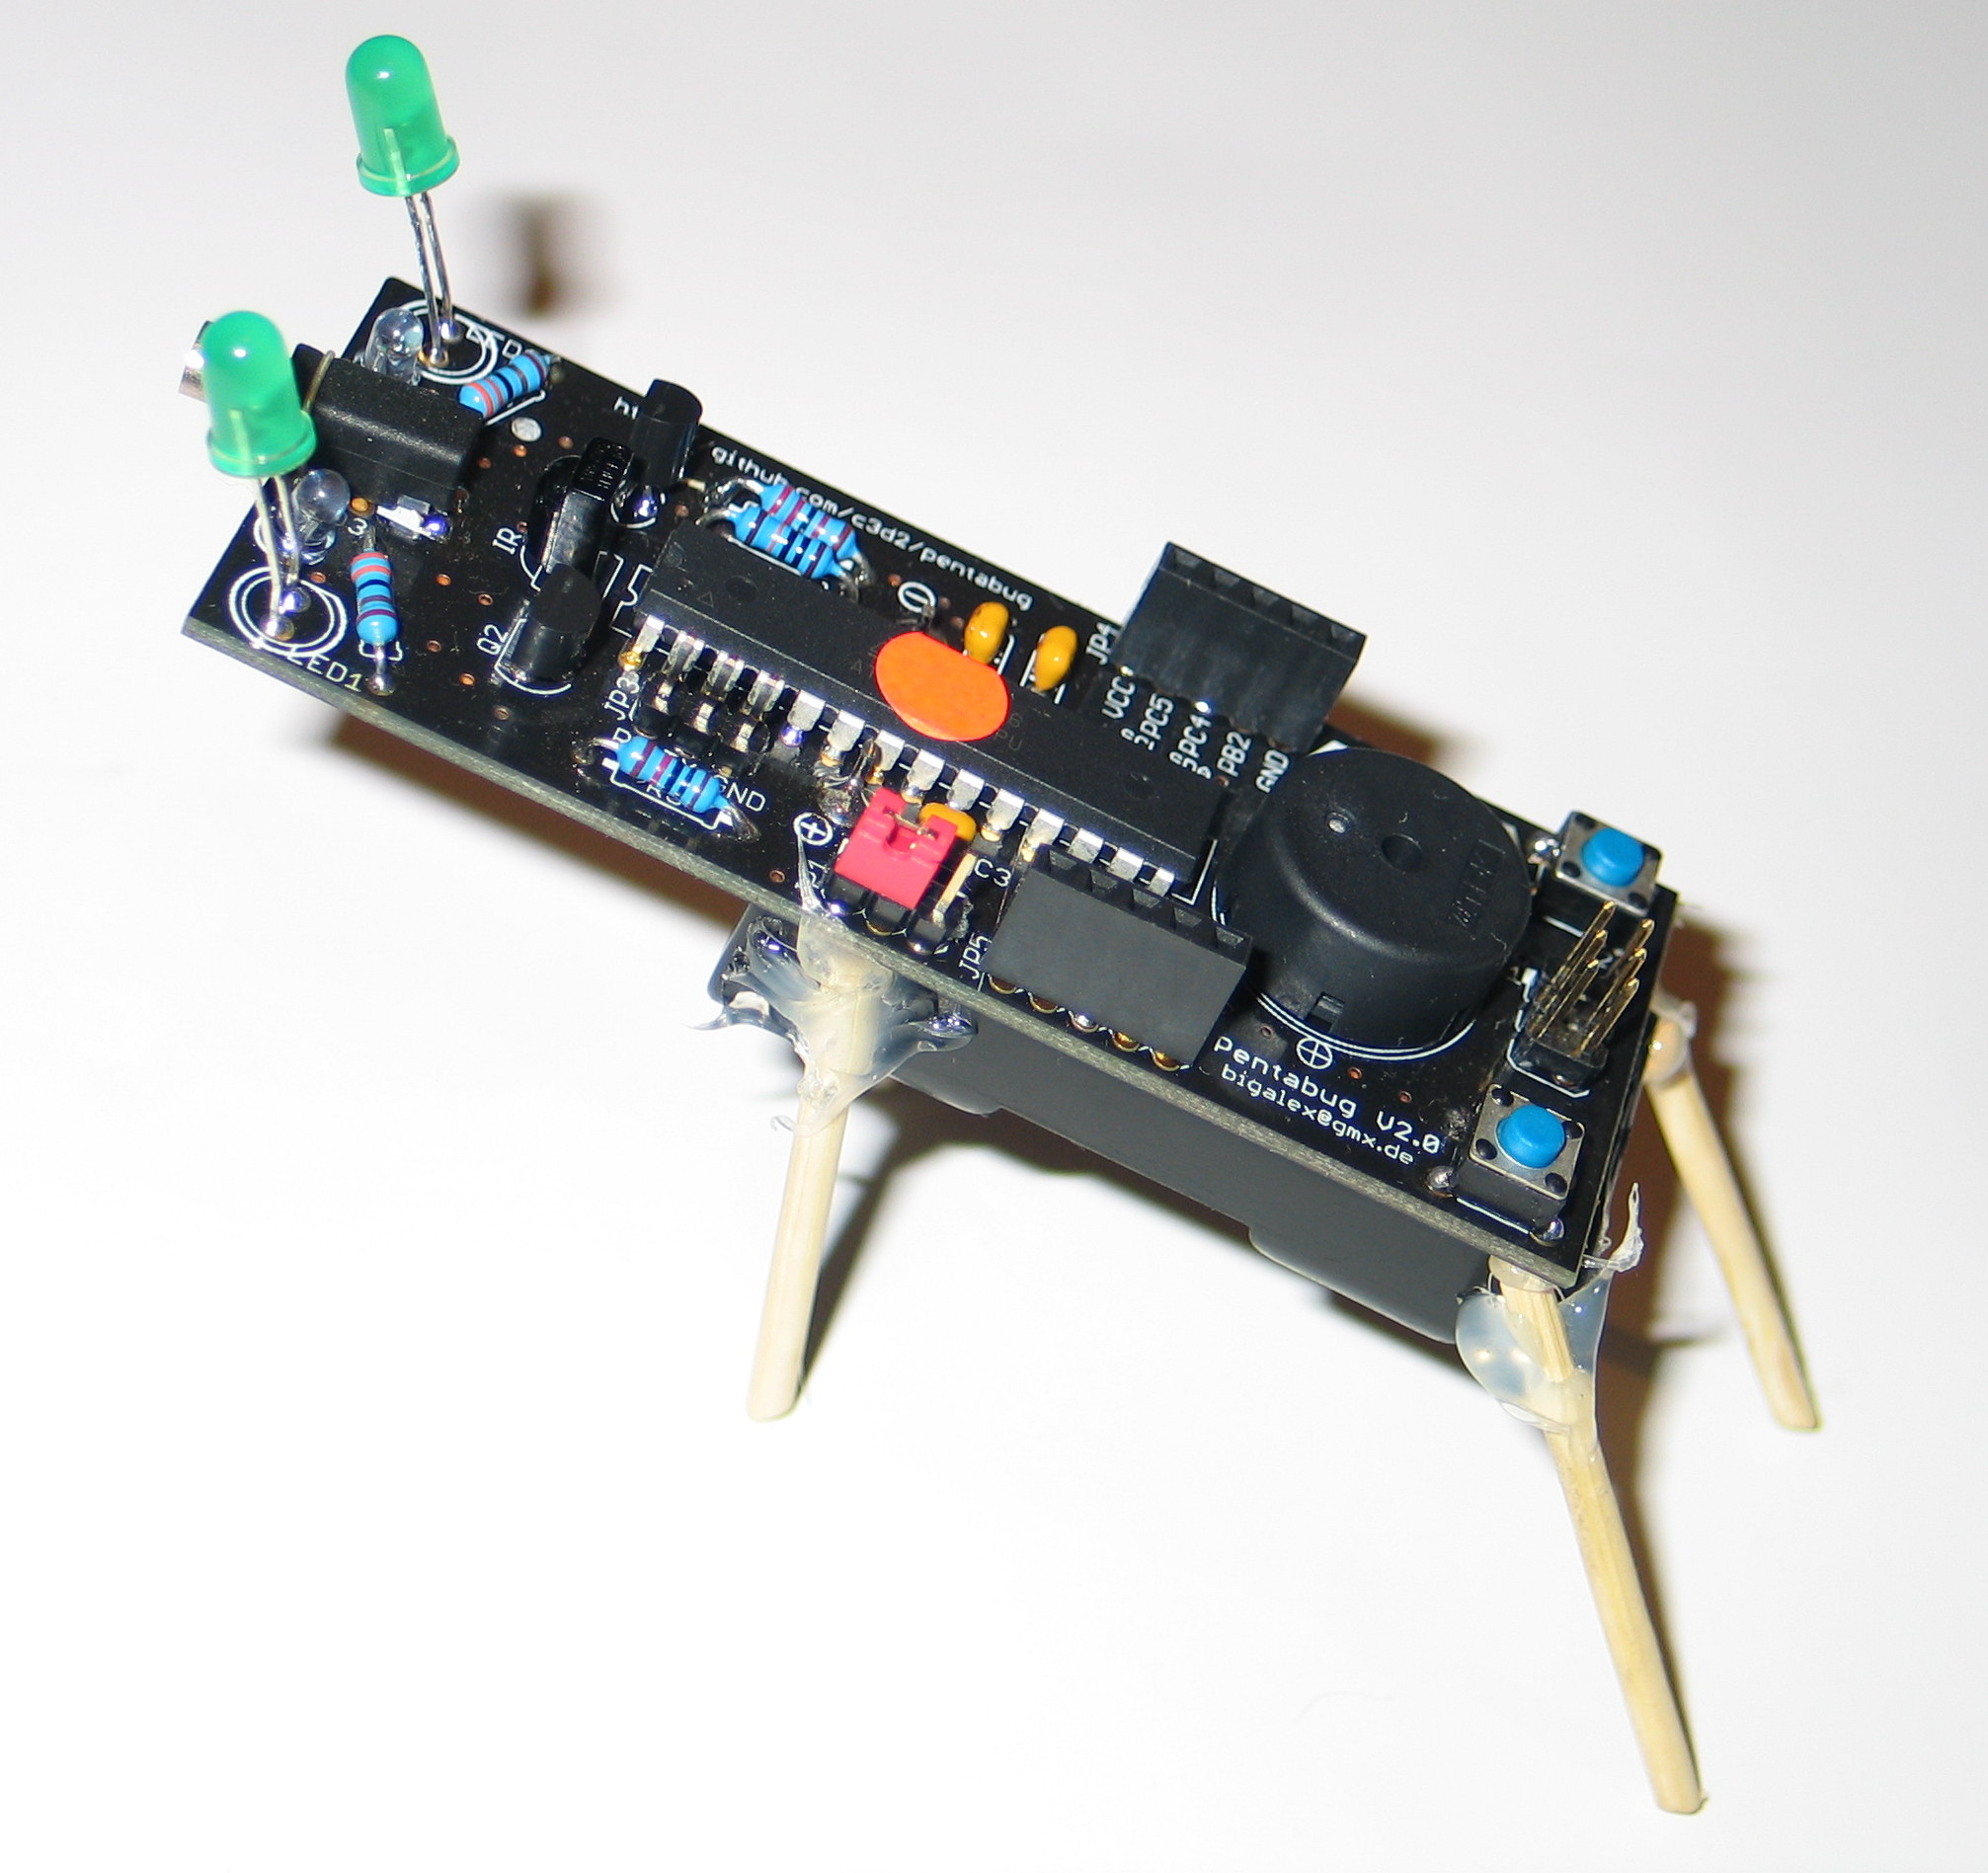
\includegraphics[height=0.7\textheight]{../img/pentabug.jpg}
			\end{center}
			}
		\only<5>{
			\begin{center}
				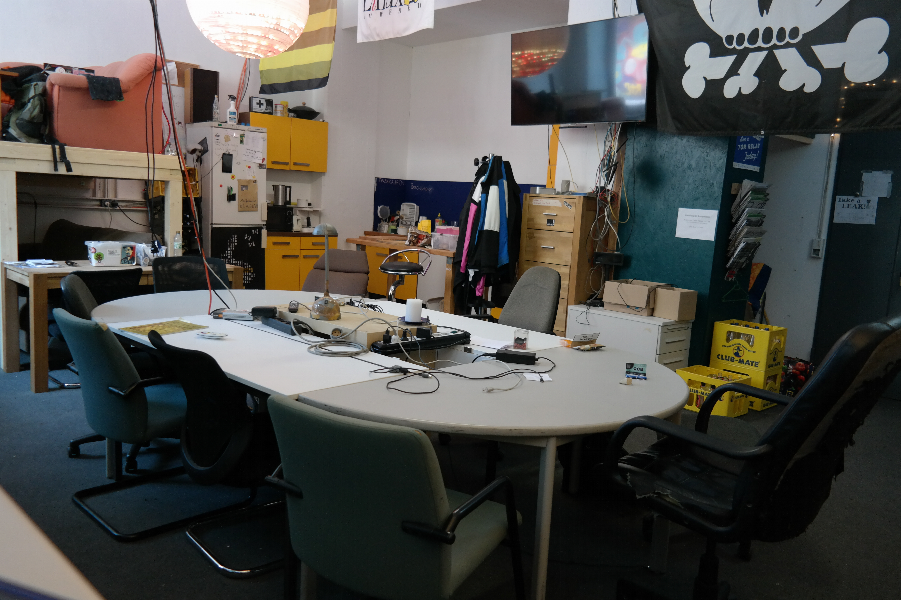
\includegraphics[height=0.7\textheight]{../img/c3d2_innen.png}			
			\end{center}
			}
		\only<6>{
			\begin{center}
				
\includegraphics[height=0.5\textheight]{../img/cms-text.png}			
			\end{center}
			}
		\only<7>{
			\begin{itemize}
				\item<1-> seit ca. 2007
				\item<2-> Ehrenamtlich organisiert
				\item<3-> Bildung und Sensibilisierung
			\end{itemize}
			}
	\end{center}
\end{frame}

\section{Internet}
\subsection{}

\begin{frame}
	\frametitle{Internet}
	\only<1>{
		\begin{center}
		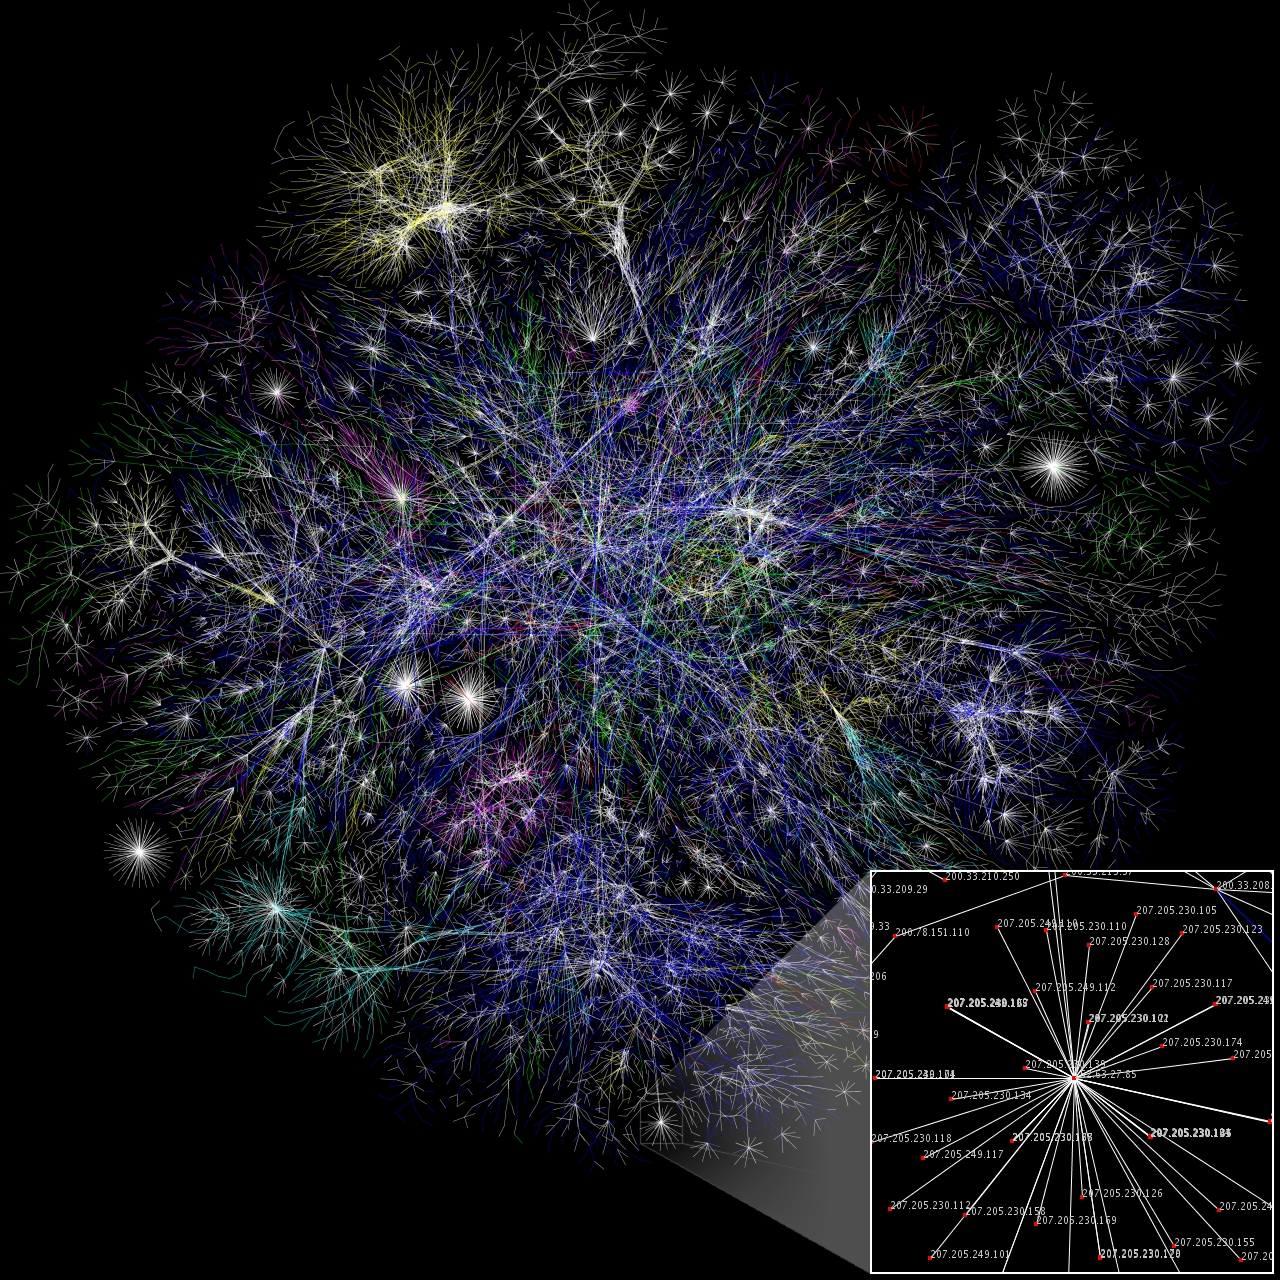
\includegraphics[height=0.7\textheight]{../img/internet_2.jpg}
		\end{center}
		}
	\only<2>{
		\begin{center}
			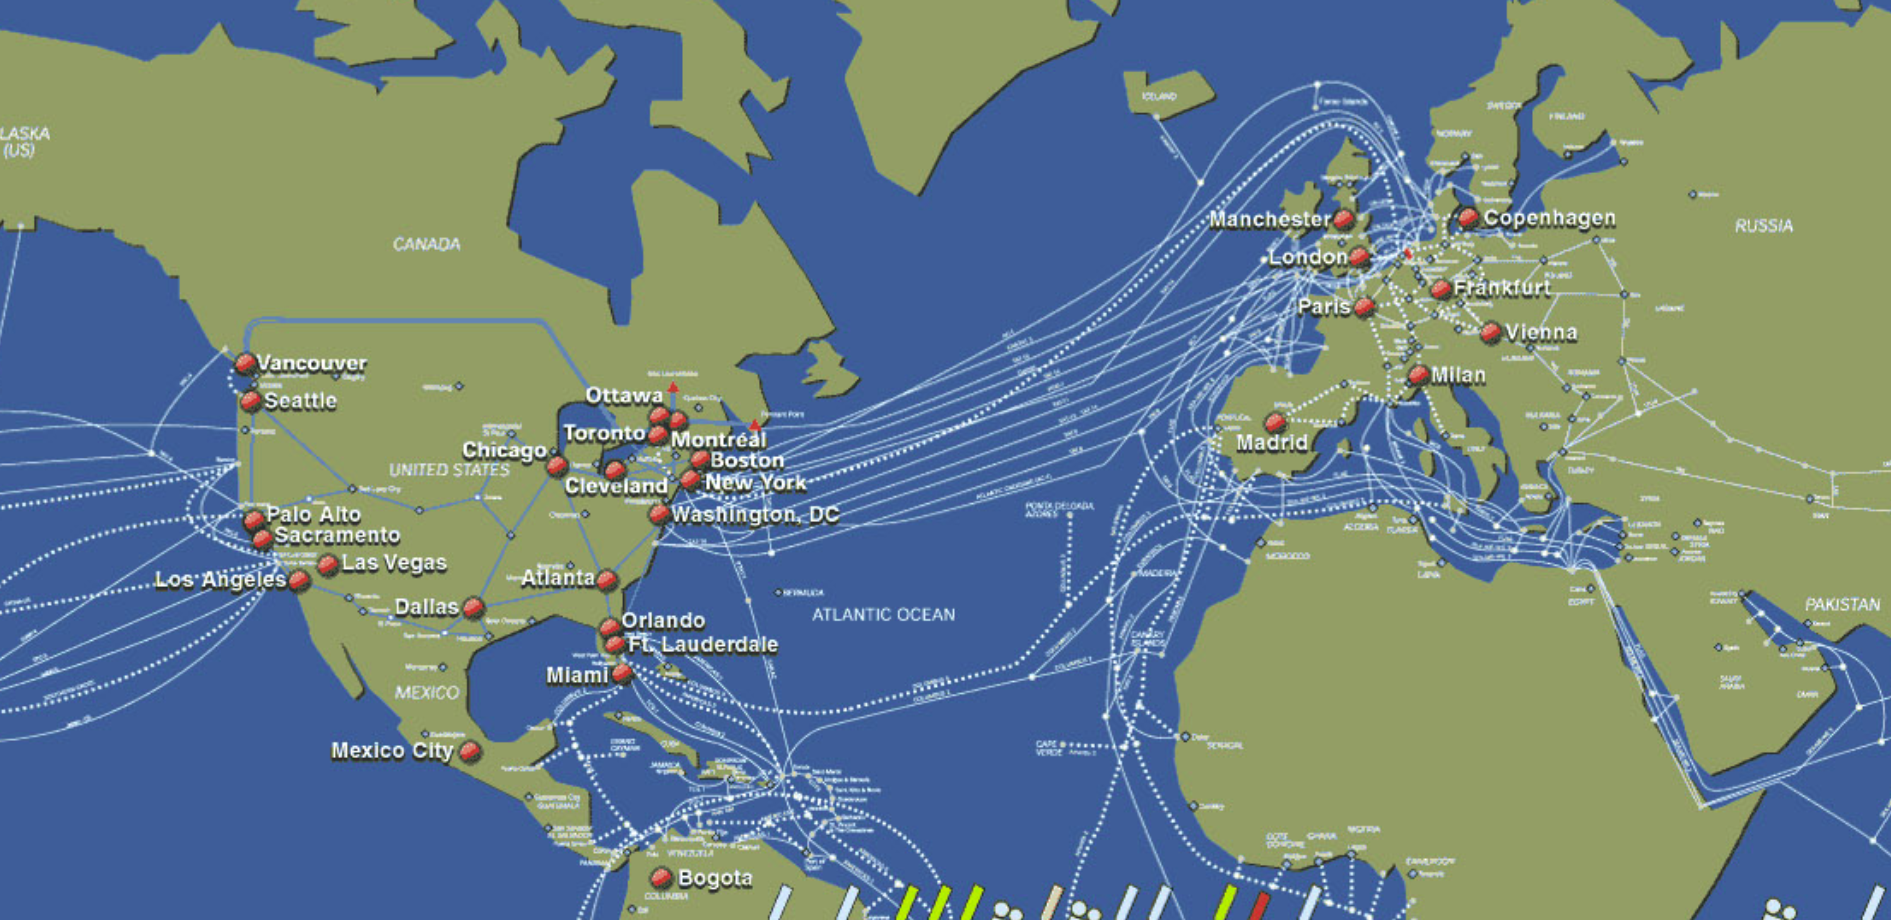
\includegraphics[height=0.5\textheight]{../img/internet_1.png}
		\end{center}
		}
\end{frame}

\section{Soziale Netzwerke}
\subsection{}

\begin{frame}
	\frametitle{Soziale Netzwerke}
	\begin{center}
		\only<1>{
			\begin{center}
				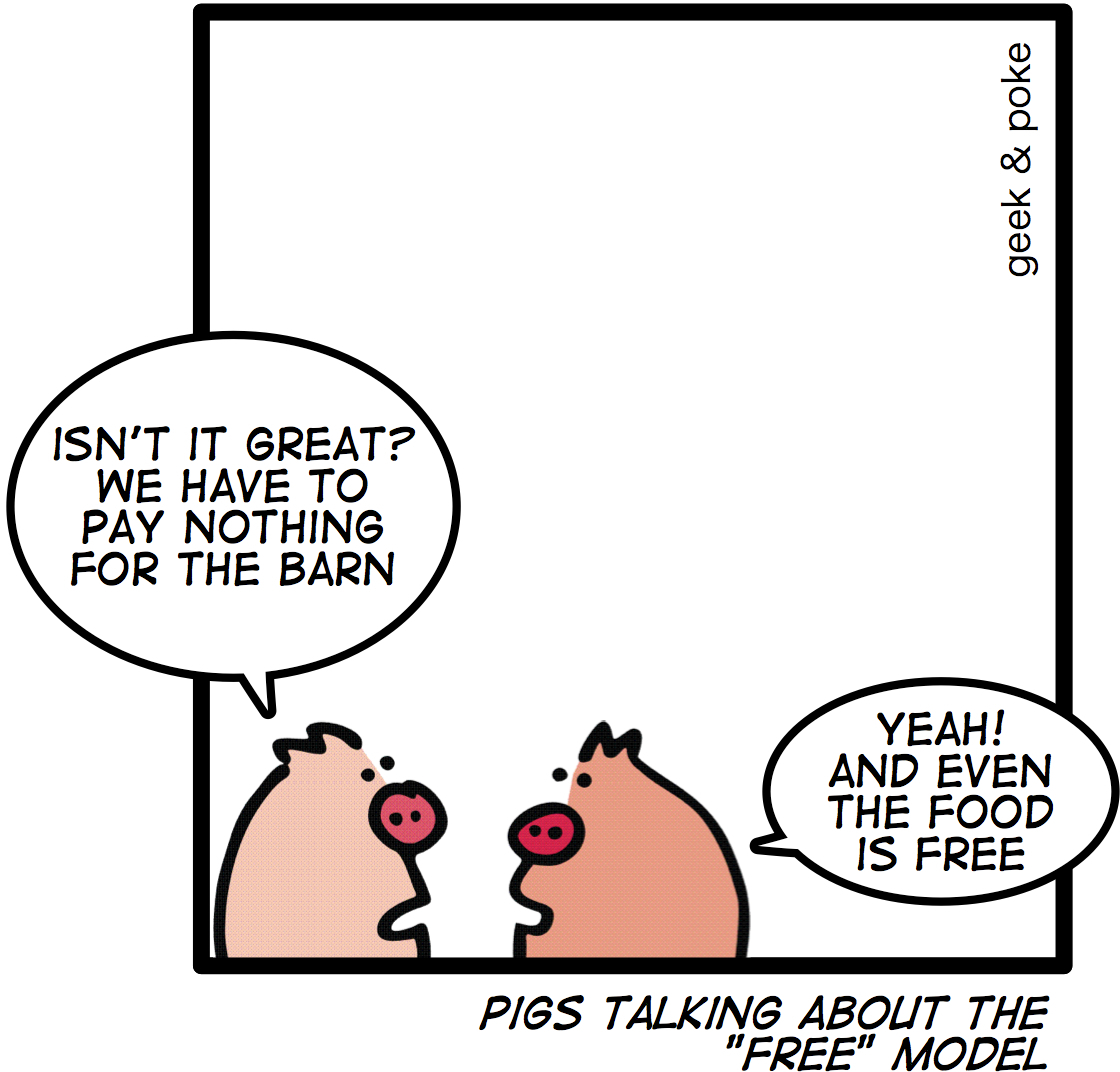
\includegraphics[height=0.7\textheight]{../img/business_pigs.jpg}
			\end{center}
			}
		\only<2>{
			Mögliche Fragen ...
			\begin{itemize}
				\item Ausdrucken?
				\item vom Balkon rufen?
			\end{itemize}
		}
	\end{center}
\end{frame}

\section{Sicherheit}
\subsection{}

\begin{frame}
    \frametitle{Passwörter}
    \begin{itemize}
        \item Keine einfachen Wörter
        \item Groß-, Kleinbuchstaben, Ziffern, Sonderzeichen
        \item Beispiele:
            \begin{itemize}
                \item dragon
                \item (nCuAj.§Tsm!f
                \item IchLiebeDich
                \item .§)=)=`
                \item 123456
            \end{itemize}
        \item<2> Verschiedene Passwörter nutzen!
    \end{itemize}
\end{frame}

\begin{frame}
  \frametitle{SSL}
  \begin{center}
      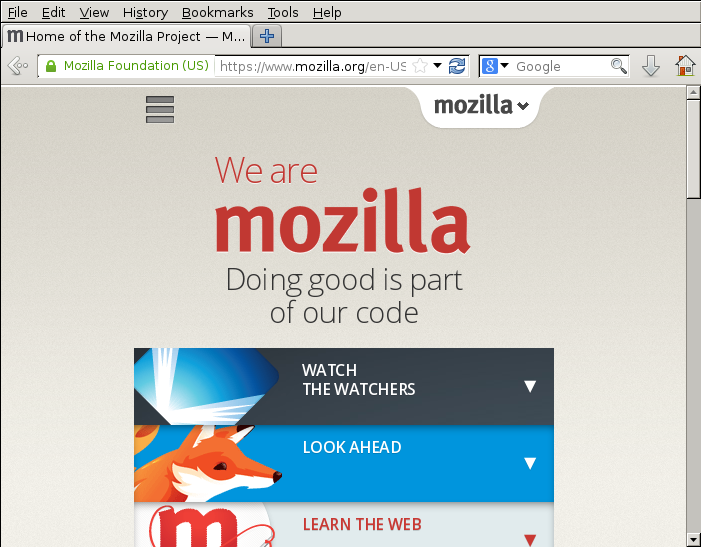
\includegraphics[height=0.7\textheight]{../img/ssl_special.png}
  \end{center}
\end{frame}

\begin{frame}
    \frametitle{Verschlüsselung: symmetrisch}
    \begin{center}
	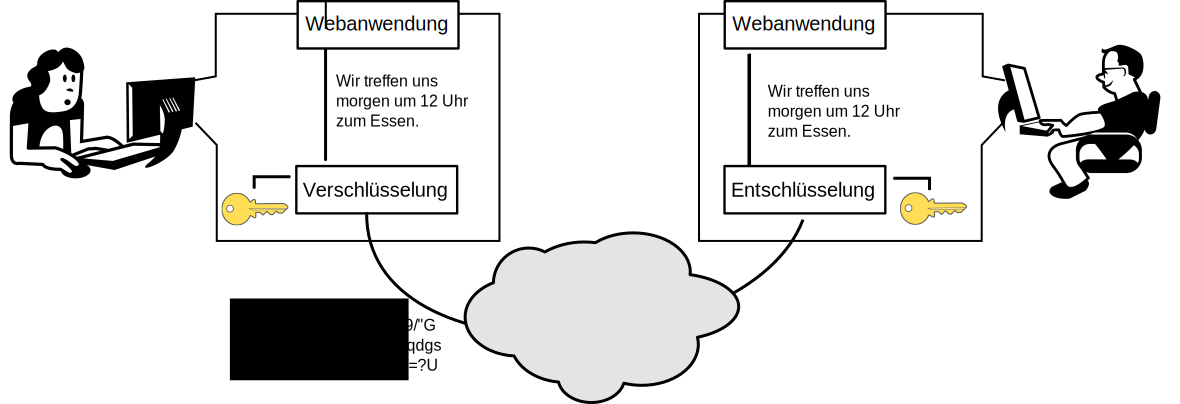
\includegraphics[width=\textwidth]{../img/krypto.pdf}
    \end{center}	
\end{frame}

\begin{frame}
    \frametitle{Verschlüsselung: asymmetrisch}
    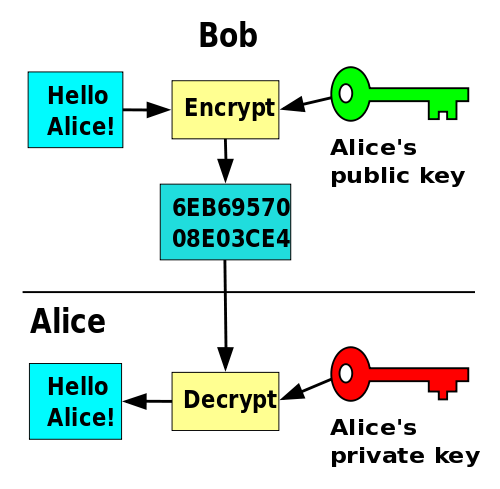
\includegraphics[height=0.7\textheight]{../img/asym_encryption.png}
\end{frame}

\begin{frame}
    \frametitle{Tracker \& Cookies}
    \begin{center}
    	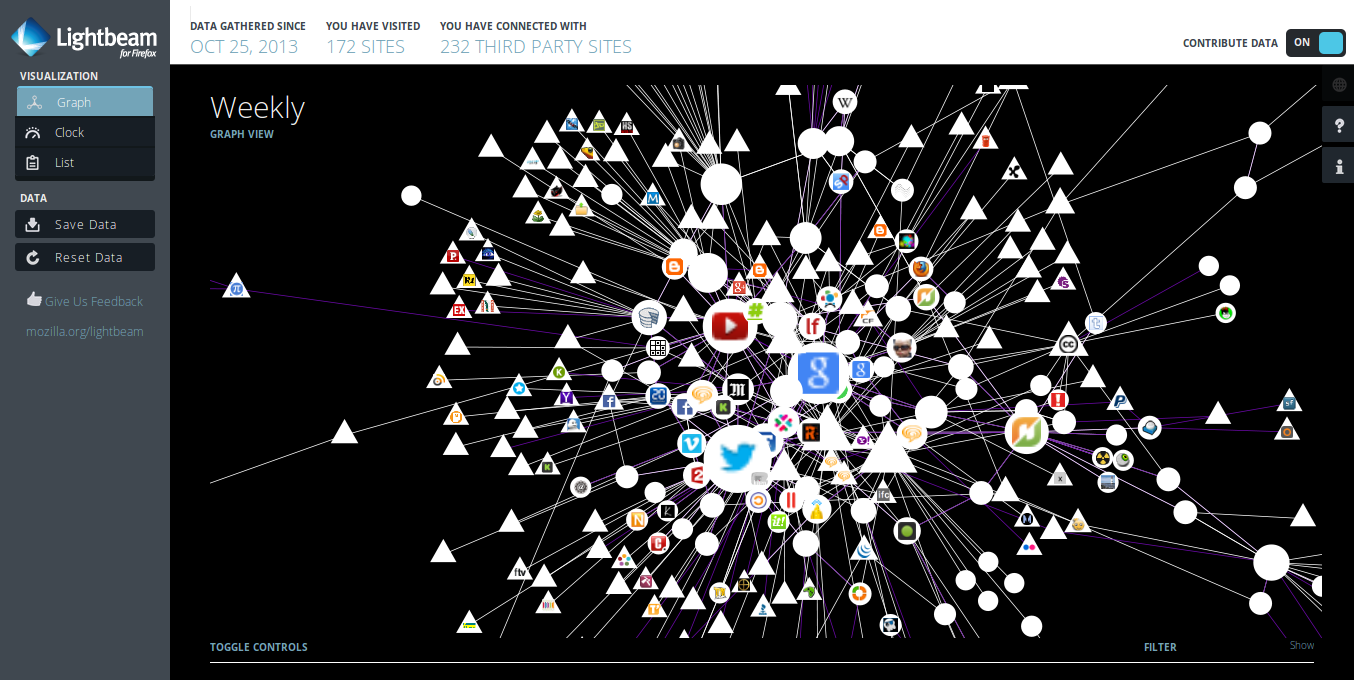
\includegraphics[height=0.7\textheight]{../img/lightbeam.png}
    \end{center}
\end{frame}

\begin{frame}
	\begin{itemize}
		\item Verlauf
	    \item Betriebssystem
    	\item Browser
      	\item Bildschirmauflösung
      	\item Plugins
      	\item Schriftarten
      	\item Zeitzone
	\end{itemize}
\end{frame}

\begin{frame}
	\frametitle{Browser Fingerprint}
	\begin{center}
	    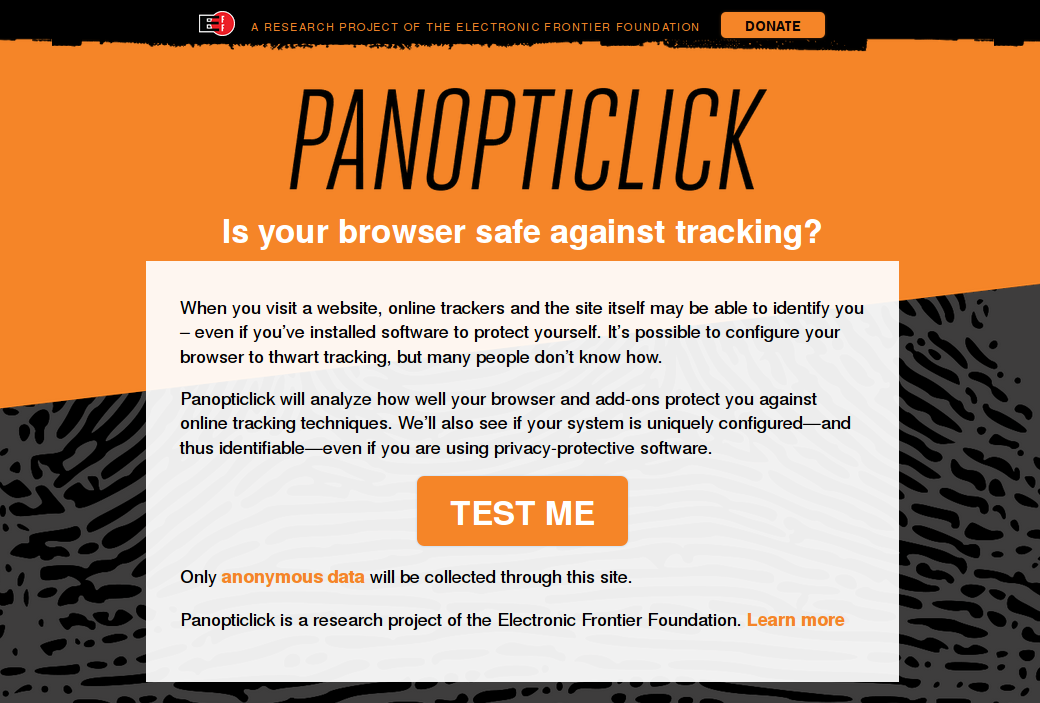
\includegraphics[height=0.7\textheight]{../img/browser_fingerprint.png}
    	\newline
    	\url{https://panopticlick.eff.org/}
    \end{center}
\end{frame}

\begin{frame}
	\frametitle{Firefox Add-ons}
    \begin{itemize}
      	\item HTTPS Everywhere
      	\item uMatrix
      	\item uBlock Origin
      	\item Lightbeam
    \end{itemize}
\end{frame}

\begin{frame}
    \frametitle{HTTPS Everywhere}
    \begin{center}
    	
\includegraphics[height=0.7\textheight]{../img/https_everywhere.png}
    \end{center}
\end{frame}

\begin{frame}
    \frametitle{uMatrix}
    \begin{center}
    	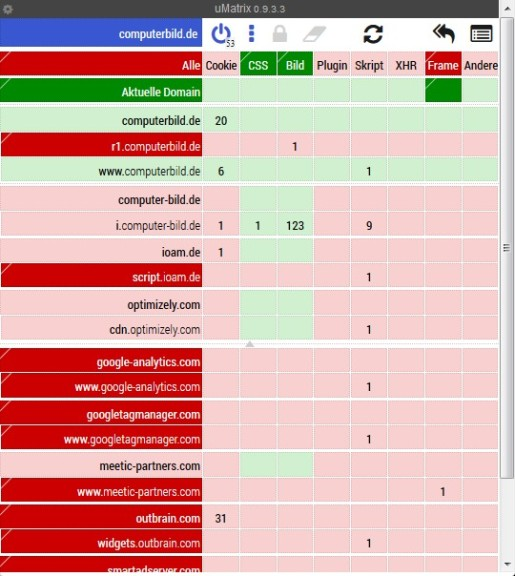
\includegraphics[height=0.7\textheight]{../img/umatrix.jpg}
    \end{center}
\end{frame}

\begin{frame}
    \frametitle{uBlock Origin}
    \begin{center}
    	
\includegraphics[height=0.7\textheight]{../img/ublock-edge-extension.png} 
	\end{center}       
\end{frame}

\begin{frame}
    \frametitle{Lightbeam}
    \begin{center}
    	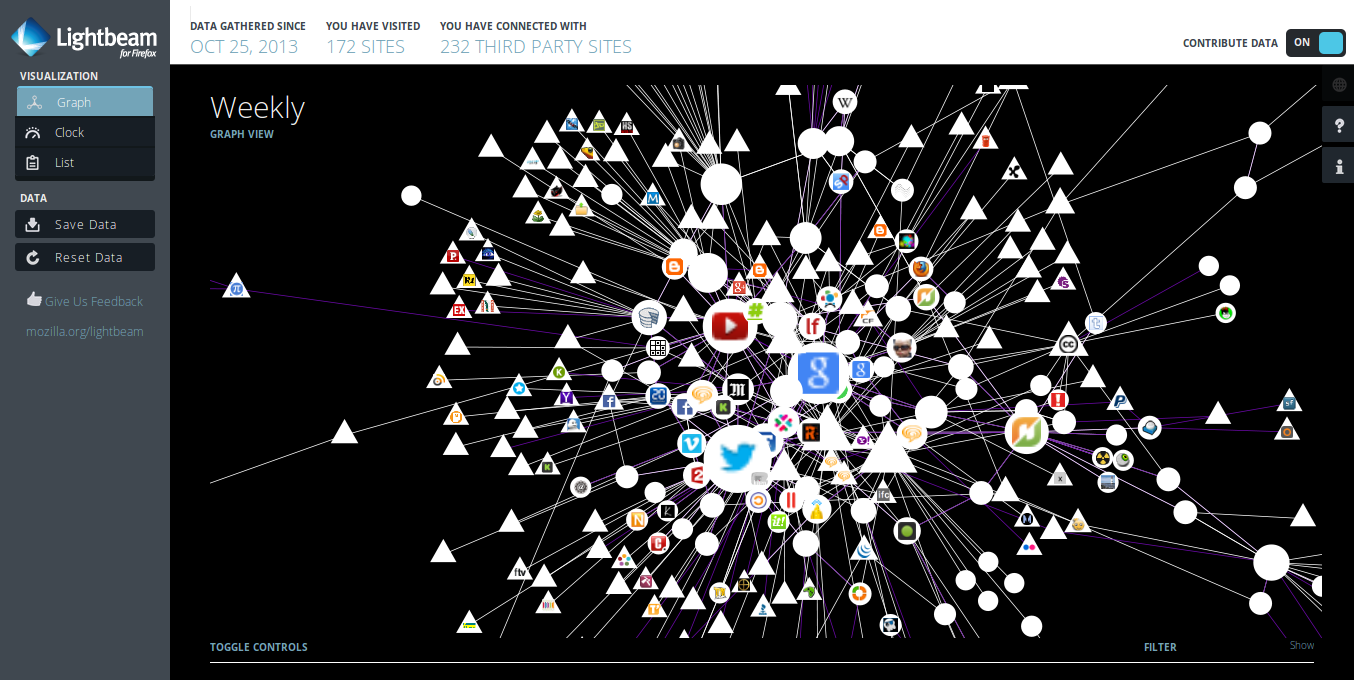
\includegraphics[height=0.7\textheight]{../img/lightbeam.png}
    \end{center}
\end{frame}

\section{Kommunikation}
\subsection{}

\begin{frame}
	\frametitle{Instant Messenger}
	Wikipedia
\end{frame}

\begin{frame}
	\frametitle{E-Mail}
	GnuPG
	\begin{itemize}
		\item Plattform unabhängig
		\item Ende zu Ende
		\item Web of Trust
	\end{itemize}
\end{frame}

\section{Filter}
\subsection{}

\begin{frame}
	\frametitle{Filter}
	\only<1>{	
		Filter sind sinnlos weil ...
		\begin{itemize}
			\item leicht zu umgehen
			\item nicht skalierbar
		\end{itemize}
	}
	\only<2>{
		Lösung?
		\begin{itemize}
			\item vorbereiten
			\item begleiten
			\item vertrauen
		\end{itemize}
	}
\end{frame}

\section{Alternativen}
\subsection{}

\begin{frame}
	\frametitle{Alternativen}
	\begin{columns}
	\column{6.5cm}
	\textbf{Freie Software}
	\begin{itemize}
		\item Betriebssystem
		\item Mobile
		\item Suchmaschinen
		\item Cloud
	\end{itemize}
	\end{columns}
\end{frame}

\begin{frame}
	\frametitle{Betriebssystem}
	\only<1>{
    	\textbf{Linux}
    	\begin{itemize}
    		\item Open Source \& Frei
      		\item hohe Anpassbarkeit
      		\item Paketverwaltung
      		\item Auswahl an Distributionen \& Desktopumgebungen
    	\end{itemize}
    }
    \only<2>{
    	\textbf{LineageOS}
    	\begin{itemize}
    		\item keine Gapps
    		\item Monatliche Updates
    		\item Unabhängigkeit
    	\end{itemize}
    }
\end{frame}

\begin{frame}
	\frametitle{Mobile}
	\begin{columns}
    \column{6.5cm}
    \textbf{F-Droid}\\
    Android-Appstore für freie Software
    
\includegraphics{../img/fdroid.png}
    \end{columns}
\end{frame}

\begin{frame}
	\frametitle{Alternative Suchmaschinen}
	\begin{columns}
		\begin{column}{5cm}
			\begin{center}
				\begin{itemize}
					\item Startpage
					\vspace{2cm}
					\item DuckDuckGo
				\end{itemize}
			\end{center}
		\end{column}
		\begin{column}{5cm}
			\begin{center}
				
\includegraphics[width=0.5\textwidth]{../img/startp_logo.png}
				\vspace{1cm}
				
\includegraphics[width=0.8\textwidth]{../img/duckduckgo.png}
			\end{center}
		\end{column}
	\end{columns}
\end{frame}

\begin{frame}{Nextcloud}
	\begin{columns}
		\column{4cm}
		\footnotesize
		Plattformübergreifende Synchronisierung von Dateien, Dokumenten, Kalendern, Kontakten, Notizen und News.
		\column{6cm}
		\begin{center}
			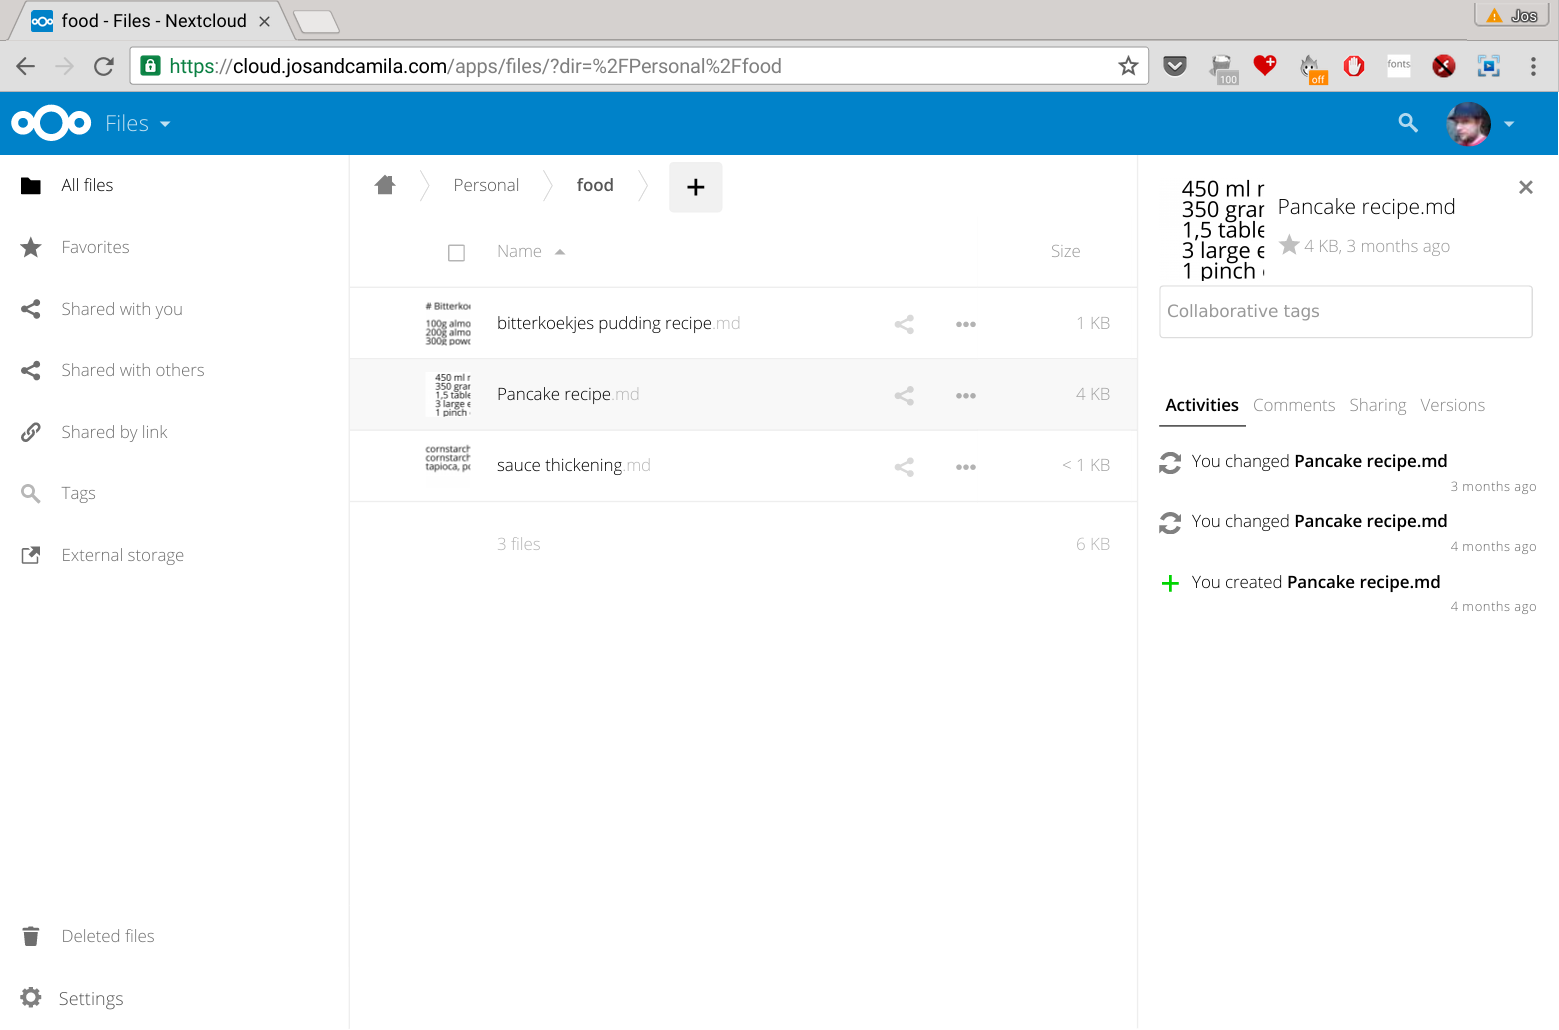
\includegraphics[width=6cm]{../img/nextcloud.png}
			\par
		\end{center}
	\end{columns}
\end{frame}

\section{Ende}
\subsection{}

\begin{frame}
	\frametitle{Ende}
	\begin{center}
		\textbf{Vielen Dank für eure Aufmerksamkeit}
	\end{center}
	\par
	\begin{columns}
		\column{3cm}
	\end{columns}
	\begin{center}
		\textbf{Kontakt}\\
		cms@lists.c3d2.de\\
		nac@c3d2.de\\
		\begin{columns}
			\column{3cm}
		\end{columns}
		\textbf{Webseite}\\
		\url{https://c3d2.de}
		\begin{columns}
			\column{3cm}
		\end{columns}
		\textbf{Termine}\\
		Datenspuren 2018\\
		22.09. - 23.09.2018\\
		\url{https://datenspuren.de/2018}
	\end{center}				
\end{frame}

\end{document}





